\newpage
\section{2023春}
\setcounter{yearcounter}{2023}

\subsection{構造工学}
\spprob{
  下に示すような、高さ$h$、幅$b$の長方形断面で、ヤング率$E$の等方線形弾性材料からなる骨組み構造について、以下の問いに答えなさい。
  ただし、すべての部材の断面積と材料は同一とする。
  また、せん断応力及びせん断変形の影響は考慮しないものとする。
  
  \begin{figure}[H]\centering
    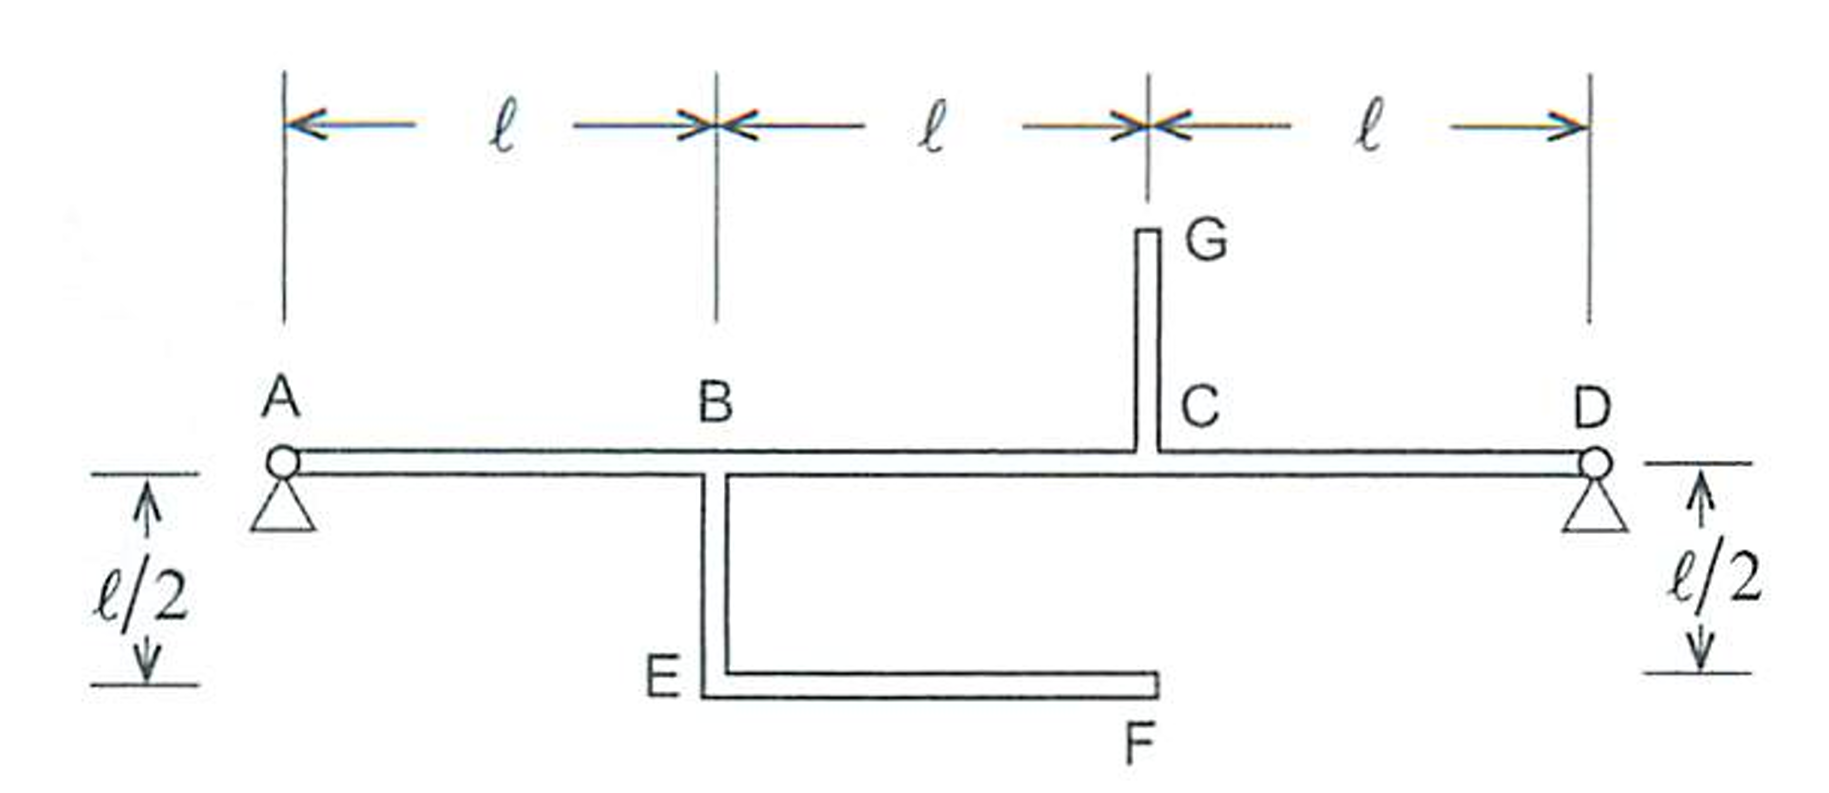
\includegraphics[width=.8\linewidth]{./src/fig/Specialized/S_2023_spring_1.png}
  \end{figure}
  
  \begin{enumerate}[label=(\arabic*)]
    \item 点Fに、反時計回りのモーメント$M_1=1$を作用させたときの曲げモーメント図を書きなさい。
    \item 問(1)の荷重条件のとき、点Cに生じる最大応力を求めなさい。ただし、長方形断面の断面二次モーメントは$bh^3/12$である。
    \item 問(1)のモーメント荷重を2倍にするとき、点Cに生じる最大応力が問(2)の値と同じになるためには部材の高さを何倍にすれば良いか答えなさい。
    \item 問(1)の荷重条件のとき、点Gの水平変位を求めなさい。
    \item 問(1)のモーメント荷重を取り除き、点Gに水平右向きの荷重$P_1=1$を与えるときの点Fの回転角を求めなさい。
    \item 問(5)の荷重条件で、点Fが回転しないように固定したときの点Fのモーメント反力を求めなさい。
  \end{enumerate}
}


\subsection{コンクリート工学}
\spprob{
\begin{enumerate}[label=\arabic*.]
  \item コンクリート用混和材について、以下の問に答えよ。
  \begin{enumerate}[label=(\arabic*)]
    \item フライアッシュをセメントに置換して使用したときに起こる反応の名称を答え、その反応の特徴を説明せよ。
    \item 高炉スラグ微粉末をセメントに置換して使用したときに起こる反応の名称を答え、その反応の特徴を説明せよ。
    \item (1)と(2)で答えた2つの反応の違いを説明せよ。
  \end{enumerate}
  \item 表は3種類のセメントに含まれるクリンカー鉱物の組成と化学組成を示している。
  表中の(a),(b),(c)は普通ポルトランドセメント、早強ポルトランドセメント、中庸熱ポルトランドセメントのいずれかである。
  (a),(b),(c)がそれぞれどのセメントであるか答え、そのように選択した理由を答えよ。
  \begin{table}[H]
  \centering
  \begin{tabular}{ccccccccc}
  \toprule
    \multicolumn{1}{c|}{セメントの} & \multicolumn{4}{c|}{クリンカー鉱物組成(\%)} & \multicolumn{4}{c}{化学組成(\%)} \\
  \cline{2-9}
    \multicolumn{1}{c|}{種別} & \ce{C3S} & \ce{C2S} & \ce{C3A} & \multicolumn{1}{c|}{\ce{C4AF}} & \ce{SiO2} & \ce{Al2O3} & \ce{Fe2O3} & \ce{CaO} \\
  \midrule
    (a) & 67 & 9 & 8 & 8 & 20.8 & 4.5 & 2.8 & 64.9 \\ 
  \midrule
    (b) & 48 & 30 & 5 & 11 & 23.3 & 3.9 & 4.0 & 63.5 \\ 
  \midrule
    (c) & 50 & 26 & 9 & 9 & 22 & 5.1 & 3.0 & 63.8 \\ 
  \bottomrule
  \end{tabular}\end{table}
  \item RCはり部材の代表的なせん断破壊形式を二つ答え、それぞれの破壊形式の特徴を説明せよ。
\end{enumerate}
}

\subsection{地盤工学}
\spprob{
\begin{enumerate}[label=\arabic*.]
  \item 矢板を打設して川底を掘削する場合について考える。
  図1は掘削現場の断面と地盤内の二次元定常流れを表した正方形フローネットを表している。
  実線と破線はそれぞれ流線と等ポテンシャル線を表している。
  地盤の透水係数は$k=2.0\tm10^{-2}\si{cm/sec}$、水の密度は$\rho_{\rm{w}}=1.0\tm10^3\si{kg/m^3}$、
  重力加速度は$g=\SI{9.8}{m/sec^2}$である。以下の問に答えよ。
  \begin{enumerate}[label=(\arabic*)]
    \item 図1の定常浸透流れを保つためには、掘削底面でポンプにより浸出する水を汲み上げる必要がある。
    奥行を\SI{1}{m}として、1日当たりの汲み上げ量を求めよ。
    \item 点Aの間隙水圧を求めよ。
    \item 掘削前に安定計算を実施したところ、ボイリングが発生する危険性が判明したとする。
    考え得る対策工法の具体例を一つ挙げよ。
  \end{enumerate}
  
  \begin{figure}[H]\centering
    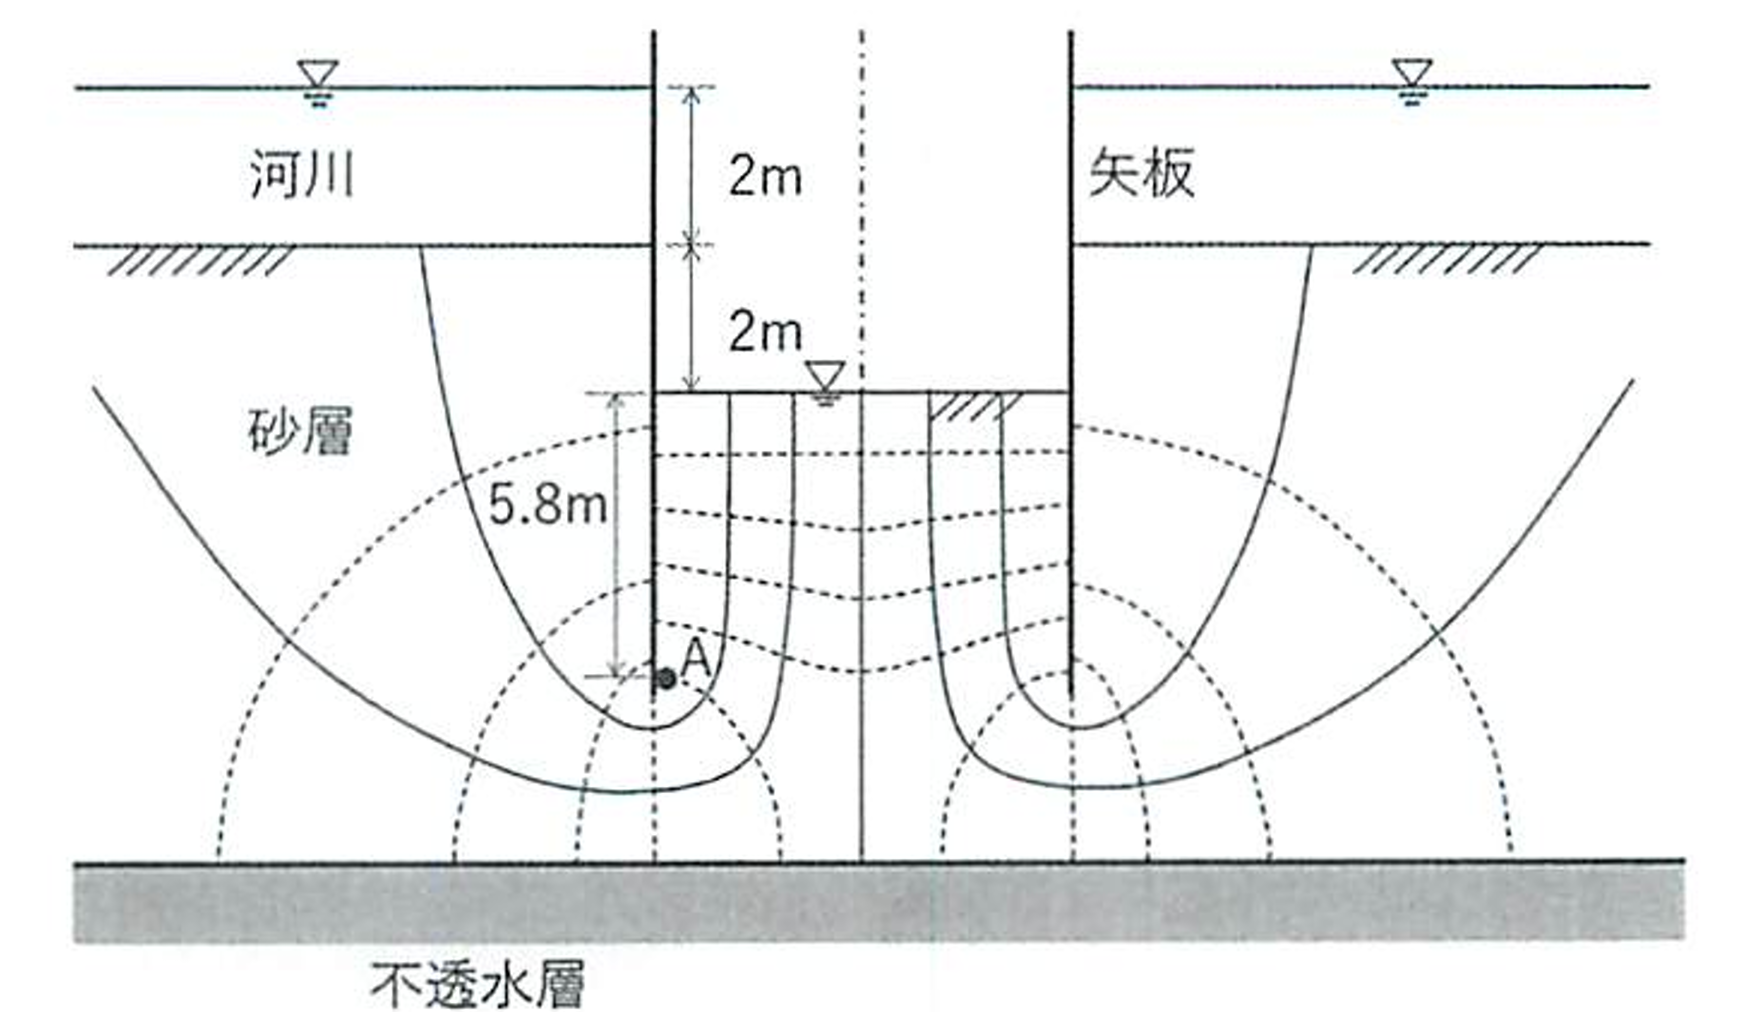
\includegraphics[width=.8\linewidth]{./src/fig/Specialized/S_2023_spring_3.png}
  \end{figure}
  
  
  \item 飽和正規圧密粘土の排水および非排水三軸圧縮試験について考える。
  せん断開始時の有効拘束圧は$p_0$であり、せん断中のセル圧は一定とする。
  飽和正規圧密粘土の有効応力に関する粘着力と内部摩擦角は、排水条件に依らず、
  $c'=0$と$\phi'$とする。
  また、鉛直応力$\grs_{\rm{v}}$と側方応力$\grs_{\rm{h}}$の差を軸差応力$q=\grs_{\rm{v}}-\grs_{\rm{h}}$
  とする。以下の問に答えよ。
  \begin{enumerate}[label=(\arabic*)]
    \item 排水三軸圧縮試験の破壊次の軸差応力$q_{\rm{d}}$を$p_0$と$\phi'$を用いて表せ。
    \item 非排水三軸圧縮試験の破壊次の軸差応力$q_{\rm{u}}$を破壊次の過剰間隙水圧$u_{\rm{f}}$と$p_0$、$\phi'$を用いて表せ。
    \item $u_{\rm{f}}$を$m$と$p_0$によって表せ。ただし、$m=q_{\rm{u}}/q_{\rm{d}}$である。
  \end{enumerate}
  
\end{enumerate}
}

